% Niveau :      PCSI *
% Discipline :  Chimie Orga I
% Mots clés :   Spectrométrie UV-visible, Réactions acidobasiques

\begin{exercise}{Magnétisme et table périodique}{3}{PCSI}
{Atomistique,Classification périodique, Structure électronique}{bermu}

\paragraph{Question ouverte :} après avoir rappelé ce qui caractérise la configuration électronique fondamentale des atomes diamagnétiques et paramagnétiques, décrire et justifier la table ci-dessous dans la mesure de vos connaissances.


    \begin{figure}[H]
        \centering
        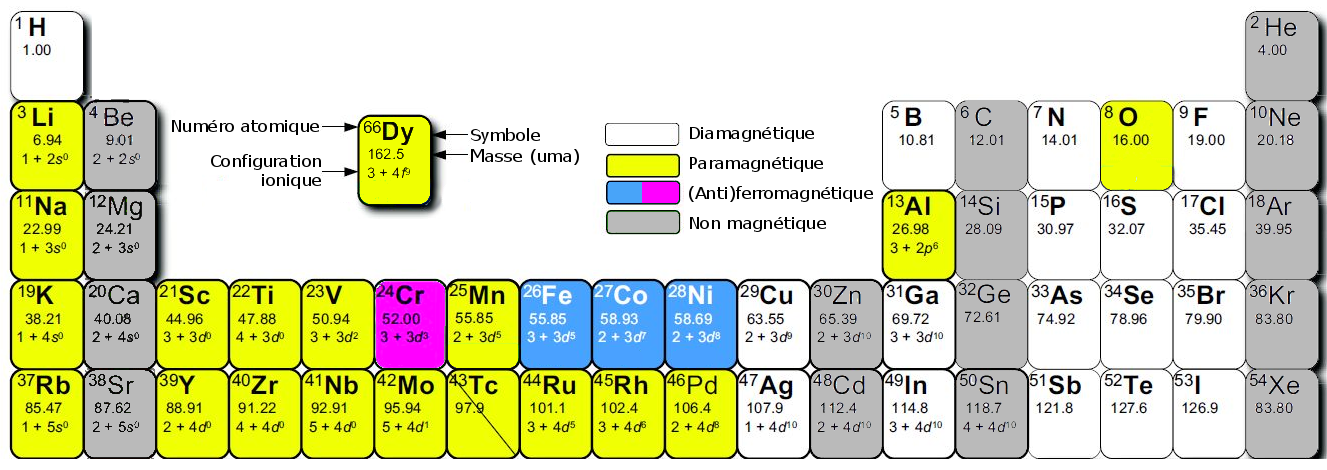
\includegraphics[width=\linewidth]{chimiePC/atomes/magnet.png}
        \caption{Propriétés magnétiques et tableau périodique}
    \end{figure}

\end{exercise}